\documentclass[a4paper,10pt]{scrartcl}
\usepackage[utf8]{inputenc}

% Title Page
\title{Lectures 1--?: Introduction to Computer Programming and Python}
\author{Andrew D. Wickert}

\usepackage{listings}
\usepackage{framed}
\usepackage{graphicx}
\lstset{mathescape,basicstyle=\ttfamily} % Allow escaping to LaTeX inside $..$

\usepackage{color}
\usepackage[hyphens]{url}
\usepackage[colorlinks=true]{hyperref}

\newcommand{\todo}[1]{\textcolor{red}{@TODO: #1}} 
 
% From http://en.wikibooks.org/wiki/LaTeX/Source_Code_Listings, modified a little

\definecolor{mygreen}{rgb}{0,0.6,0}
\definecolor{mygray}{rgb}{0.5,0.5,0.5}
\definecolor{mymauve}{rgb}{0.58,0,0.82}

\lstset{ %
  backgroundcolor=\color{white},   % choose the background color; you must add \usepackage{color} or \usepackage{xcolor}
  basicstyle=\scriptsize,          % the size of the fonts that are used for the code
  breakatwhitespace=false,         % sets if automatic breaks should only happen at whitespace
  breaklines=true,                 % sets automatic line breaking
  captionpos=b,                    % sets the caption-position to bottom
  commentstyle=\color{mygreen},    % comment style
  deletekeywords={...},            % if you want to delete keywords from the given language
  escapeinside={\%*}{*)},          % if you want to add LaTeX within your code
  extendedchars=true,              % lets you use non-ASCII characters; for 8-bits encodings only, does not work with UTF-8
  frame=single,                    % adds a frame around the code
  keepspaces=true,                 % keeps spaces in text, useful for keeping indentation of code (possibly needs columns=flexible)
  keywordstyle=\color{blue},       % keyword style
  language=Python,                 % the language of the code
  morekeywords={*,...},            % if you want to add more keywords to the set
  numbers=left,                    % where to put the line-numbers; possible values are (none, left, right)
  numbersep=5pt,                   % how far the line-numbers are from the code
  numberstyle=\tiny\color{mygray}, % the style that is used for the line-numbers
  rulecolor=\color{black},         % if not set, the frame-color may be changed on line-breaks within not-black text (e.g. comments (green here))
  showspaces=false,                % show spaces everywhere adding particular underscores; it overrides 'showstringspaces'
  showstringspaces=false,          % underline spaces within strings only
  showtabs=false,                  % show tabs within strings adding particular underscores
  stepnumber=2,                    % the step between two line-numbers. If it's 1, each line will be numbered
  stringstyle=\color{mymauve},     % string literal style
  tabsize=2,                       % sets default tabsize to 2 spaces
  title=\lstname                   % show the filename of files included with \lstinputlisting; also try caption instead of title
}

\begin{document}
\maketitle

\section{Why do we program computers?}

In order to analyze data, run simulations, check the logical consistency of our ideas, and compare models to the real world, we need numbers. Working with numbers requires quite a lot of repetitive calculation. Doing these calculations ourselves is boring, miserable, and saps our very humanity. Fortunately, computers are excellent at doing repeated tasks. Automating a computer to do our ``dirty work'' is what programming is all about. In order to send instructions to the computer, we need to write in a language that obeys rules of unambiguous formal logic. This is a computer programming language.

Over this course, there will be many struggles in making this communication between you and the computer work. Therefore, it is important to remember why we program computers: these reasons include to make our lives easier and more pleasant, to accomplish more than we could without the assistance of a computer, to have a perfectly logical companion who can inform us about the internal consistency of our ideas, and to build a numerical laboratory in which we can develop virtual experiments. If it seems that computers are making our lives harder rather than easier, it is time to take a step back and a deep breath, and evaluate what we are doing and why we are doing it.

\section{How we program computers}

Computer programming languages are a set of commands that we write in human-readable text that eventually are turned into machine-readable binary. This can happen via one of two means:
\begin{itemize}
 \item In a \textbf{compiled language}, we use a program called a ``compiler'' to translate what we have written into machine language. In the past, this was done by hand -- so you can thank your lucky stars for all of the dedicated engineers, mathematicians, programmers, and technicians who have made these compilers that literally tell a computer how to program itself based on your commands to it!
 \item In an \textbf{interpreted language} (or ``scripting language''), your commands are not compiled into byte code (machine language) \textit{en masse}. Rather, they all reference pre-compiled functions. Because of this, you don't have to re-compile the program every time you change it and your coding can be very flexible, but these programs often run somewhat slower than compiled programs. This is the trade-off: ease of programming for you costs computational efficiency in this case.
\end{itemize}

\begin{figure}[h]
\begin{center}
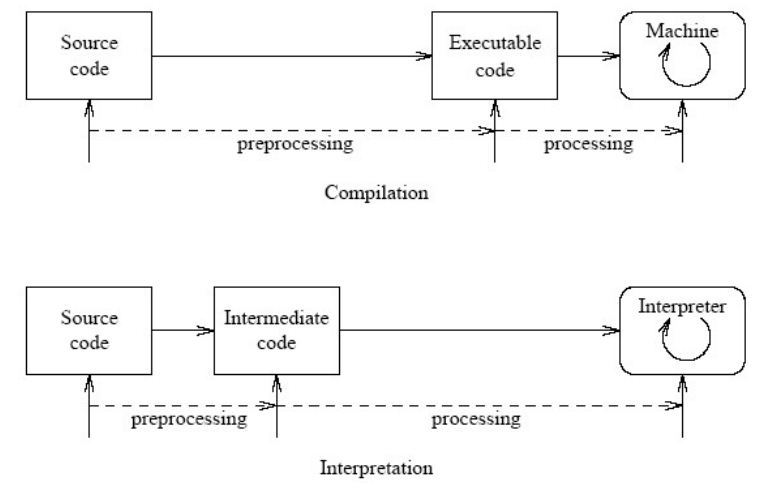
\includegraphics[width=.8\linewidth]{figures/Introduction/Compilervrsinterpreter.JPG}
\end{center}
\caption{Compiltered languages are pre-processed (i.e. compiled) for efficiency for the computer (but not the human!). Interpreted languages are processed at runtime -- one less step for developers (i.e. humans), but more effort for the computer. Image from Aniket Thakur at \url{http://opensourceforgeeks.blogspot.com/2013/03/difference-between-compiler-interpreter.html}.}
\end{figure}

\section{Python and the major programming languages}

In this course, we will learn Python. It is an interpreted, multi-paradigm, multi-purpose, and easy-to-read open-source language. These mean that:
\begin{itemize}
 \item \textbf{Interpreted:} You don't have to compile the code every time you make a change. This helps speed code development and your learning (critical in this course!) at the cost of some computational efficiency (*not* critical in this course).
 \item \textbf{Multi-paradigm:} This means that the language can be written as an \textbf{imperative} language, with a sequence of command that are executed in some defined order, or as an \textbf{object-oriented language}, in which ``objects''---clusters of related variables and functions: think perhaps of a volume of soil that has a temperature and thermal conductivity (variables) and can conduct heat (a function)---are manipulated.
 \item \textbf{Multi-purpose:} Python cam be used for numerical modeling, data analysis, web development, interfacing with peripheral devices, automating tasks in GIS, and much more.
 \item \textbf{Easy-to-read:} As programming languages go, Python can be ``read'' fairly well by someone who has no experience with it.
 \item \textbf{Open-source:} Python is freely available and is updated and expanded by a dedicated community of volunteers. Therefore, learning how to use it will not tie your skills to any software package that must be purchased.
\end{itemize}
Many of these reasons highlight why I have chosen to work with Python for this course. However, it is important to go over a number of the other major programming languages used in the geosciences, at very least such that their names are familiar to you and you will not feel like you are starting from nothing if you have to program in one of them someday. These are:

\begin{figure}
\begin{center}
\begin{tabular}{l|c|c}
 & \textbf{Compiled} & \textbf{Interpreted} \\
\hline
\textbf{Open-source} & \begin{tabular}{@{}c@{}}Fortran \\ C/C++ \\ Java\end{tabular} & \begin{tabular}{@{}c@{}}Python \\ R \\ Octave (Matlab clone)\end{tabular}  \\
\hline
\textbf{Proprietary} & C\# \\ Swift & \begin{tabular}{@{}c@{}}Matlab \\ IDL \end{tabular}
\end{tabular}
\end{center}
\caption{Open-source and proprietary, interpreted and compiled, programming languages. For open-access and ease-of-use, we will be using Python, which is interpreted and open-source.}
\end{figure}

C, C++, and Fortran (f77 and f95) are the most commonly-used compiled programming langauges for scientific computing. These are the true ``heavy lifters'' in computational science. Fortunately, Python is written in C (giving it a native interface with C code), and a compiler called ``f2py'' allows Fortran code to be compiled in such a way that Python can talk to it. Java is occasionally used, but is less developed in the numerical realm.

Many of your colleagues in the general geosciences use Matlab, which is a very similar language, except that it is more focused on matrix operations, data analysis, and scientific computing... and that it is closed-source, meaning that you cannot see how it actually works. Furthermore, you need to purchase a license to use it. For those of you who are familiar with Matlab already, I would suggest the Mathesaurus entry ``Numpy for Matlab Users'' (Numpy is the numerical package for Python) at \url{http://mathesaurus.sourceforge.net/matlab-numpy.html}.

IDL is commonly used by atmospheric scientists as well as the community involved with the ENVI GIS package. However, the other major GIS packages, both proprietary (ArcGIS) and open-source (GRASS GIS and QGIS) use Python as their interface language.

R is a programming language designed to perform statistical analyses. It excels in this field. However, outside of this scope, it is fairly limited, which is why we won't learn it in this course. After learning Python, learning R should be straightforward.

The other reasons to teach you Python are that it has functions that streamline file input and output and can connect easily to programs written in other languages, including compiled langauges, making it an effective language to ``glue'' together pieces of code written in highly efficient (but clunkier to manipulate) C or Fortran code. It also produces excellent graphical outputs. In short, what I am writing that I have chosen Python after thinking long and hard about the decision and using it for an extended period of time myself, and I think that learning it will be a worthwhile use of your time.

\section{Practical interlude: downloading and installing}

\subsection{Python interpreter and development environment}

Now we know that we can write code in Python that can be interpreted into a machine language. Great! So how does that happen?

With an interpreter, of course! You must download and install one onto your computer. Linux/*nix and Mac computers come pre-loaded with a basic Python interpreter, but we will need more packages than that, and the Mac version of the Python interpreter is often not up-to-date. Windows machines generally do not come with Python by default.

While the interpreter changes human-readable text into machine language, it does not help humans produce that human-readable text. This is where a development environment comes in. This is something that will format the text for us to help us follow the flow of the code, automatically complete expressions, and more. There are a two main options to do this:

\begin{itemize}
 \item Command prompt and text editor. In each of these cases, I recommend \textbf{ipython} as the program to execute the Python code at the command line interface (= command prompt). Some examples of combinations of these are:
 \begin{itemize}
  \item Windows: Cygwin and notepad++
  \item Linux: Terminal and gedit
  \item Mac: Terminal and textwrangler
 \end{itemize}
 \item Spyder: a Matlab-like Integrated Development Environment (IDE)
\end{itemize}

Shell and text editor: gedit/notepad++/textwrangler and ipython or Spyder


The Python packages that we will want at the outset of this course are:
\begin{itemize}
 \item The most recent Python 2.*.* (not Python 3.* -- this is a fairly different take on Python that is not connected to the scientific programming packages)
 \item NumPy (\textbf{Num}erical \textbf{Py}thon): a package to handle arrays, matrix operations, and more
 \item SciPy (\textbf{Sci}entific \textbf{Py}thon): a package that contains special functions, interpolation techniques, linear algebra solvers, and other tools that are useful for scientific programming
 \item Matplotlib: a plotting library with an extensive range of applications (see \url{http://matplotlib.org/gallery.html}); we \todo{will} use the map-plotting extensions to matplotlib later in this course.
\end{itemize}

\subsubsection{Linux}

Use your package manager. For Debian/Ubuntu, type at the command line:

\begin{lstlisting}[language=sh]
# Basic packages
sudo apt-get install \
python python-numpy python-scipy \
python-setuptools python-matplotlib 

# pip (recommended for automatic installs via setuptools)
sudo apt-get install python-pip

# iPython console -- very useful (optional)
sudo apt-get install ipython

# Sypder IDE (I don't personally use it but many others like it: optional)
sudo apt-get install spyder
\end{lstlisting}

(The package ``python'' should be installed by default\footnote{Once I was trying to change which version of Python I was using, and without thinking about it (or knowing nearly so much as I do now), I simply typed ``sudo apt-get remove python'' and entered my password and pressed enter. However, had I looked at the screen to see the list of packages that  would also be removed, I would have realized that the list of core functions of my computer that depend on the Python interpreter was enormous. Long story short: had to reboot to a command-line terminal to ``apt-get install'' and put all of the core software back on my computer, just so I could boot to the desktop!}, but is included in this list for completeness.)

\subsubsection{Windows}

Download \textbf{python(x,y)} (\url{https://code.google.com/p/pythonxy/wiki/Downloads}) or another full-featured distribution such as \textbf{Anaconda}; both of these distributions have been tested successfully with gFlex. Python(x,y), Anaconda, and several others also contain the required packages (including the numerical libraries), the iPython console, and the Spyder IDE; \textbf{Spyder} (\url{https://code.google.com/p/spyderlib/}) is a nice IDE that will provide a familiar-looking interface for users accustomed to Matlab.

\subsubsection{Mac}

One recommendation is to use a package manager like \textbf{homebrew} (\url{http://brew.sh/}). With this you can install Python, and then move on to using \textbf{pip} (or homebrew) to install the Python modules. A good introduction to this can be found here: \url{http://www.thisisthegreenroom.com/2011/installing-python-numpy-scipy-matplotlib-and-ipython-on-lion}. See the \textbf{Linux} instructions for the list of packages that you will need; after installing pip, these commands can be substituted as follows, e.g.,

\begin{lstlisting}[language=sh]
# Homebrew
sudo brew install python-numpy
# Pip
pip install numpy
\end{lstlisting}

Recent efforts to download Python distributions (both **Anaconda** and **Enthought**) have not met with success with both gFlex and GRASS, though **Anaconda** has been tested successfully with Windows. As a result, it should be more successful to keep the Python packages managed better by something like **homebrew** with **pip**.

\section{Letters and numbers:A look from the computer's point of view}

ASCII, binary, Unicode, int, uint, floating point

Python does automatic typing *but* it is important to know these for general programming!

\section{Basic Python programming}

The following sections provide a brief introduction to programming in Python. A more exhaustive treatment can be found in the textbook, \emph{Think Python: How to Think Like a Computer Scientist} (PDF and HTML available at \url{http://www.greenteapress.com/thinkpython/}).

\subsection{So you want to write a program}

By now, you know that a program is a set of user-readable text that the computer can understand and use to drive its actions. Even though at this point you might not be familiar with a program, immersion is a way of learning, so here is a simple program that we will use for examples in the next several sections.

\begin{lstlisting}[belowskip=-1.6\baselineskip, language=python]

#! /usr/bin/env python

# firstExample.py
# 
# Written by ADW on 05 May 2015
# while finishing these notes at the last minute
# (as usual) to teach class tomorrow
# 
# This program will continue adding numbers to a starting
# value until the number reaches 50.
# It then multiplies this by 2 three times.

import sys

counter = 0 # value to be modified

while counter < 50:
  counter += 1

if counter == 50:
  # It should at this point!
  print "50!"
else:
  print "Error!"
  
for i in range(3):
  # i = [0, 1, 2] (0-indexing)
  counter *= 10

if counter == 50 * 10**3:
  print "Checks out -- done!"
  print "Final counter =", counter
else:
  sys.exit("Fail!")
  
print "Now let's divide counter by 25001, just over half"
print counter/25001

print "Now let's divide counter by 25001., just over half"
print counter/25001.

\end{lstlisting}

Before going any further, I will make a note of a couple of pieces of this code here:
\begin{lstlisting}[belowskip=-1.6\baselineskip, language=python]

#! /usr/bin/env python
\end{lstlisting}
This is the ``shebang''. It is important on Unix-like operating systems (e.g., Linux, Mac) to tell the computer which interpreter to use.

Next,
\begin{lstlisting}[belowskip=-1.6\baselineskip, language=python]

#! /usr/bin/env python

# firstExample.py
# 
# Written by ADW on 05 May 2015
# while finishing these notes at the last minute
# (as usual) to teach class tomorrow
# 
# This program will continue adding numbers to a starting
# value until the number reaches 50.
# It then multiplies this by 2 three times.
\end{lstlisting}
The pound sign (hashtag!), \#, denotes comments. These can be used throughout your code. And they should be used! Many hours of work writing code are often rendered useless when someone else tries to use it only to find no comments among a pile of expressions in a computer language. Even worse, many people have been known to not recognize their own code 6 months or 1 year out unless they have written good comments. Get in a habit of writing many good comments early, and you will be better-off for it.

\begin{framed}
For comments, see Downey, p. 19
\end{framed}

In comments, I typically write the name of the code (in case I change it later -- to remember), the date that I started to write it (and perhaps other dates of significant code development), and my name or initials. I also write a short note about what the program does.

After this, there is ``import'' call.
\begin{lstlisting}[belowskip=-1.6\baselineskip, language=python]

import sys
\end{lstlisting}
``import'' brings in a specific package of extra functions in Python. This is called a ``module''. Eventually, when you write programs, you may create your own modules that are related to the problems that you like to solve. Such a module may relate to, for example, solutions for stress inside the Earth. The module ``sys'', as its name suggests, connects to the computer system. Towards the end of the code,
\begin{lstlisting}[belowskip=-1.6\baselineskip, language=python]

  sys.exit("Fail!")
\end{lstlisting}
causes the program to crash if it is executed. This can be useful to provide an useful message to the user if something is badly wrong. Modules have many helpful functions, most of which do not abruptly terminate the operation!

\subsection{Variables and basic types}

\begin{framed}
See Downey, pp. 13--15
\end{framed}

Variables can be things like:
\begin{lstlisting}
a = 152 # Integer (int)
b = 16.2 # "Floating point" number (float)
c = 'Ada Lovelace' # Character string (str)
d = True # Boolean (bool)
\end{lstlisting}

Each of these three examples is a different variable \textbf{type}, as noted in the comment (\# sign) after each entry. They behave differently. As might be expected, integers and floats play with each other better than do strings. The other important piece in the above code is the use of \textbf{=} as the \emph{assignment operator}. It assigns the value to that particular variable letter. This is quite powerful, as variables can allow a code to be flexible and work with a wide range of input values -- or even input types!

So now, in our above code, we can see that we have defined the variable ``counter'', and that it is an integer.
\begin{lstlisting}[belowskip=-1.6\baselineskip, language=python]

counter = 0 # value to be modified
\end{lstlisting}

What if we had wanted to make it a floating-point number? Well, we simply would put a decimal point after it.
\begin{lstlisting}[belowskip=-1.6\baselineskip, language=python]

counter2 = 0.
\end{lstlisting}

This is important when you want to take advantage of the ways in which integers and floating point numbers differ. See Section \ref{s:math} for a common example of this.

Types apply to all values in a code, whether they are assigned to variables or just added ``on the fly'' to the code.

Boolean values can be \lstinline{True} or \lstinline{False}. These are often used for ``flow control'', or telling your code how to step from one step to another. This is explained further in section \ref{s:loops}.

\subsection{Loops: for, while}
\label{s:loops}

Loops repeat execution of a piece of code while a particular condition is met. In the above code:
\begin{lstlisting}[belowskip=-1.6\baselineskip, language=python]

while counter < 50:
  counter += 1
\end{lstlisting}
changes ``counter'' by adding 1 to it so long as ``counter'' is less than 50. Pretty simple right? Well, what if we changed it to this?
\begin{lstlisting}[belowskip=-1.6\baselineskip, language=python]

trouble = True
while trouble == True:
  counter += 1
\end{lstlisting}
``=='' is the logical equals expression; while ``='' assigns values, ``=='' checks for equivalency. Would the prgram ever end?

\begin{framed}
\textbf{The power of CTRL+C (Control+C, Strg+C):} It doesn't just copy text! It forcibly terminates your programs. Very useful for stopping mistakes from getting out of hand. Like infinite loops.
\end{framed}

Would this code create an infinite loop?
\begin{lstlisting}[belowskip=-1.6\baselineskip, language=python]

trouble = True
while trouble:
  counter += 1
\end{lstlisting}
Here, we are missing the \lstinline{== True} after \lstinline{Trouble}. However, this still works. Why is that? Well, the code simply evaluates whether the statement is nonzero when trying to decide whether to continue the \lstinline{while} loop. Consider \lstinline{while counter < 50} above, for example. An additional helpful piece of information: Boolean \lstinline{True} is 1 (and \lstinline{False} is 0).

Another type of loop is a \lstinline{for} loop, in which the loop runs until you run out of values in a list. For example:
\begin{lstlisting}[belowskip=-1.6\baselineskip, language=python]
for i in range(3):
  # i = [0, 1, 2] (0-indexing)
  counter *= 10
\end{lstlisting}
\lstinline{range} is a special Python command that creates a set of values that goes up to (but does not exceed) the value inside the parentheses. So, as the comment notes, \lstinline{range(3)} produces \lstinline{[0, 1, 2]}. These square brackets indicate that this is a \lstinline{list}, a variable type that is a container for other values; this is discussed in section \ref{s:containerTypes}.

``Nesting'' is the process of combining multiple for loops. You may use the below space to write an example of nested loops and to write some thoughts about why you might want to do this.

\vspace{6cm}

\subsection{Logical operators and flow control: if, else if, else, and, or}

\begin{framed}
 See Chapter 5 in Downey for a much more thorough introduction
\end{framed}

Two portions of the code above use ``if'' and ``else''. This provides ``flow control'' for the code by giving causing events to be based on some set of inputs. In this case, it is fairly simple, but you can imagine much more complex trees of nested if/else loops.

\begin{lstlisting}[belowskip=-1.6\baselineskip, language=python]
if counter == 50:
  # It should at this point!
  print "50!"
else:
  print "Error!"
\end{lstlisting}
  
\begin{lstlisting}[belowskip=-1.6\baselineskip, language=python]
if counter == 50 * 10**3:
  print "Checks out -- done!"
  print "Final counter =", counter
else:
  sys.exit("Fail!")
\end{lstlisting}

\subsection{Exceptions: try and except}

You may use \lstinline{try} and \lstinline{except} in a way that is similar to the logical operators. This takes an action that you knnow might fail in the \lstinline{try} portion, and instead of crashing the code, ``catches'' it and moves on to the \lstinline{except} portion.

\begin{framed}
 See pages 162-163 (Downey)
\end{framed}

\subsection{``Print'' and other statements}

\begin{framed}
See Downey, p. 15
\end{framed}

\lstinline{print} sends the output to the screen. Try it! You can print several things on the same line by separating them with commans, as is accomplished in the second line of the above code, reproduced here:
\begin{lstlisting}[belowskip=-1.6\baselineskip, language=python]
  print "Checks out -- done!"
  print "Final counter =", counter
\end{lstlisting}
  
\subsection{Operators: Mathematical and String}
\label{s:math}

\begin{framed}
See Downey, p. 16, 18
\end{framed}

Operators work on numbers how you would expect; please see Downey about how they work with strings (or just experiment!). Also, note this code from above with regard to variable type:
\begin{lstlisting}[belowskip=-1.6\baselineskip, language=python]
print "Now let's divide counter by 25001, just over half"
print counter/25001

print "Now let's divide counter by 25001., just over half"
print counter/25001.
\end{lstlisting}
When an integer is divided by another integer, the code always rounds down. When there is a floating point number involved, it then gives a more exact solution.

\subsection{Types that combine several items: lists, tuples, Numpy arrays}
\label{s:containerTypes}

\subsection{Variables are references}

\begin{lstlisting}
 
\end{lstlisting}



\subsection{Why does this all work? How do computers work?}



\section{Writing programs}


\subsection{imperative}

\subsubsection{Without functions}

\subsubsection{With functions}

\subsection{Object-oriented}






\end{document}          
